\documentclass[twoside]{book}

% Packages required by doxygen
\usepackage{fixltx2e}
\usepackage{calc}
\usepackage{doxygen}
\usepackage[export]{adjustbox} % also loads graphicx
\usepackage{graphicx}
\usepackage[utf8]{inputenc}
\usepackage{makeidx}
\usepackage{multicol}
\usepackage{multirow}
\PassOptionsToPackage{warn}{textcomp}
\usepackage{textcomp}
\usepackage[nointegrals]{wasysym}
\usepackage[table]{xcolor}

% Font selection
\usepackage[T1]{fontenc}
\usepackage[scaled=.90]{helvet}
\usepackage{courier}
\usepackage{amssymb}
\usepackage{sectsty}
\renewcommand{\familydefault}{\sfdefault}
\allsectionsfont{%
  \fontseries{bc}\selectfont%
  \color{darkgray}%
}
\renewcommand{\DoxyLabelFont}{%
  \fontseries{bc}\selectfont%
  \color{darkgray}%
}
\newcommand{\+}{\discretionary{\mbox{\scriptsize$\hookleftarrow$}}{}{}}

% Page & text layout
\usepackage{geometry}
\geometry{%
  a4paper,%
  top=2.5cm,%
  bottom=2.5cm,%
  left=2.5cm,%
  right=2.5cm%
}
\tolerance=750
\hfuzz=15pt
\hbadness=750
\setlength{\emergencystretch}{15pt}
\setlength{\parindent}{0cm}
\setlength{\parskip}{0.2cm}
\makeatletter
\renewcommand{\paragraph}{%
  \@startsection{paragraph}{4}{0ex}{-1.0ex}{1.0ex}{%
    \normalfont\normalsize\bfseries\SS@parafont%
  }%
}
\renewcommand{\subparagraph}{%
  \@startsection{subparagraph}{5}{0ex}{-1.0ex}{1.0ex}{%
    \normalfont\normalsize\bfseries\SS@subparafont%
  }%
}
\makeatother

% Headers & footers
\usepackage{fancyhdr}
\pagestyle{fancyplain}
\fancyhead[LE]{\fancyplain{}{\bfseries\thepage}}
\fancyhead[CE]{\fancyplain{}{}}
\fancyhead[RE]{\fancyplain{}{\bfseries\leftmark}}
\fancyhead[LO]{\fancyplain{}{\bfseries\rightmark}}
\fancyhead[CO]{\fancyplain{}{}}
\fancyhead[RO]{\fancyplain{}{\bfseries\thepage}}
\fancyfoot[LE]{\fancyplain{}{}}
\fancyfoot[CE]{\fancyplain{}{}}
\fancyfoot[RE]{\fancyplain{}{\bfseries\scriptsize Generated on Sat Jan 16 2016 19\+:06\+:43 for Arnie\+Boids by Doxygen }}
\fancyfoot[LO]{\fancyplain{}{\bfseries\scriptsize Generated on Sat Jan 16 2016 19\+:06\+:43 for Arnie\+Boids by Doxygen }}
\fancyfoot[CO]{\fancyplain{}{}}
\fancyfoot[RO]{\fancyplain{}{}}
\renewcommand{\footrulewidth}{0.4pt}
\renewcommand{\chaptermark}[1]{%
  \markboth{#1}{}%
}
\renewcommand{\sectionmark}[1]{%
  \markright{\thesection\ #1}%
}

% Indices & bibliography
\usepackage{natbib}
\usepackage[titles]{tocloft}
\setcounter{tocdepth}{3}
\setcounter{secnumdepth}{5}
\makeindex

% Hyperlinks (required, but should be loaded last)
\usepackage{ifpdf}
\ifpdf
  \usepackage[pdftex,pagebackref=true]{hyperref}
\else
  \usepackage[ps2pdf,pagebackref=true]{hyperref}
\fi
\hypersetup{%
  colorlinks=true,%
  linkcolor=blue,%
  citecolor=blue,%
  unicode%
}

% Custom commands
\newcommand{\clearemptydoublepage}{%
  \newpage{\pagestyle{empty}\cleardoublepage}%
}


%===== C O N T E N T S =====

\begin{document}

% Titlepage & ToC
\hypersetup{pageanchor=false,
             bookmarks=true,
             bookmarksnumbered=true,
             pdfencoding=unicode
            }
\pagenumbering{roman}
\begin{titlepage}
\vspace*{7cm}
\begin{center}%
{\Large Arnie\+Boids \\[1ex]\large 0.\+0.\+1 }\\
\vspace*{1cm}
{\large Generated by Doxygen 1.8.10}\\
\vspace*{0.5cm}
{\small Sat Jan 16 2016 19:06:43}\\
\end{center}
\end{titlepage}
\clearemptydoublepage
\tableofcontents
\clearemptydoublepage
\pagenumbering{arabic}
\hypersetup{pageanchor=true}

%--- Begin generated contents ---
\chapter{Hierarchical Index}
\section{Class Hierarchy}
This inheritance list is sorted roughly, but not completely, alphabetically\+:\begin{DoxyCompactList}
\item Circle\+Shape\begin{DoxyCompactList}
\item \contentsline{section}{Star}{\pageref{class_star}}{}
\end{DoxyCompactList}
\item \contentsline{section}{Collision\+System}{\pageref{class_collision_system}}{}
\item Convex\+Shape\begin{DoxyCompactList}
\item \contentsline{section}{Bullet}{\pageref{class_bullet}}{}
\begin{DoxyCompactList}
\item \contentsline{section}{Missile}{\pageref{class_missile}}{}
\end{DoxyCompactList}
\item \contentsline{section}{Ship}{\pageref{class_ship}}{}
\begin{DoxyCompactList}
\item \contentsline{section}{Asteroid}{\pageref{class_asteroid}}{}
\item \contentsline{section}{Player}{\pageref{class_player}}{}
\item \contentsline{section}{Swarm\+Boid}{\pageref{class_swarm_boid}}{}
\end{DoxyCompactList}
\end{DoxyCompactList}
\item \contentsline{section}{Game}{\pageref{class_game}}{}
\item \contentsline{section}{Key\+Input}{\pageref{class_key_input}}{}
\item View\begin{DoxyCompactList}
\item \contentsline{section}{Camera}{\pageref{class_camera}}{}
\end{DoxyCompactList}
\item \contentsline{section}{X\+Controller}{\pageref{class_x_controller}}{}
\end{DoxyCompactList}

\chapter{Class Index}
\section{Class List}
Here are the classes, structs, unions and interfaces with brief descriptions\+:\begin{DoxyCompactList}
\item\contentsline{section}{\hyperlink{class_asteroid}{Asteroid} }{\pageref{class_asteroid}}{}
\item\contentsline{section}{\hyperlink{class_bullet}{Bullet} }{\pageref{class_bullet}}{}
\item\contentsline{section}{\hyperlink{class_camera}{Camera} }{\pageref{class_camera}}{}
\item\contentsline{section}{\hyperlink{class_collision_system}{Collision\+System} }{\pageref{class_collision_system}}{}
\item\contentsline{section}{\hyperlink{class_game}{Game} }{\pageref{class_game}}{}
\item\contentsline{section}{\hyperlink{class_key_input}{Key\+Input} }{\pageref{class_key_input}}{}
\item\contentsline{section}{\hyperlink{class_missile}{Missile} }{\pageref{class_missile}}{}
\item\contentsline{section}{\hyperlink{class_player}{Player} }{\pageref{class_player}}{}
\item\contentsline{section}{\hyperlink{class_ship}{Ship} \\*Base \hyperlink{class_ship}{Ship} class. Abstract class that inherits from sf\+::\+Convex\+Shape. Contains members common to all ships }{\pageref{class_ship}}{}
\item\contentsline{section}{\hyperlink{class_star}{Star} }{\pageref{class_star}}{}
\item\contentsline{section}{\hyperlink{class_swarm_boid}{Swarm\+Boid} }{\pageref{class_swarm_boid}}{}
\item\contentsline{section}{\hyperlink{class_x_controller}{X\+Controller} }{\pageref{class_x_controller}}{}
\end{DoxyCompactList}

\chapter{Class Documentation}
\hypertarget{class_asteroid}{}\section{Asteroid Class Reference}
\label{class_asteroid}\index{Asteroid@{Asteroid}}
Inheritance diagram for Asteroid\+:\begin{figure}[H]
\begin{center}
\leavevmode
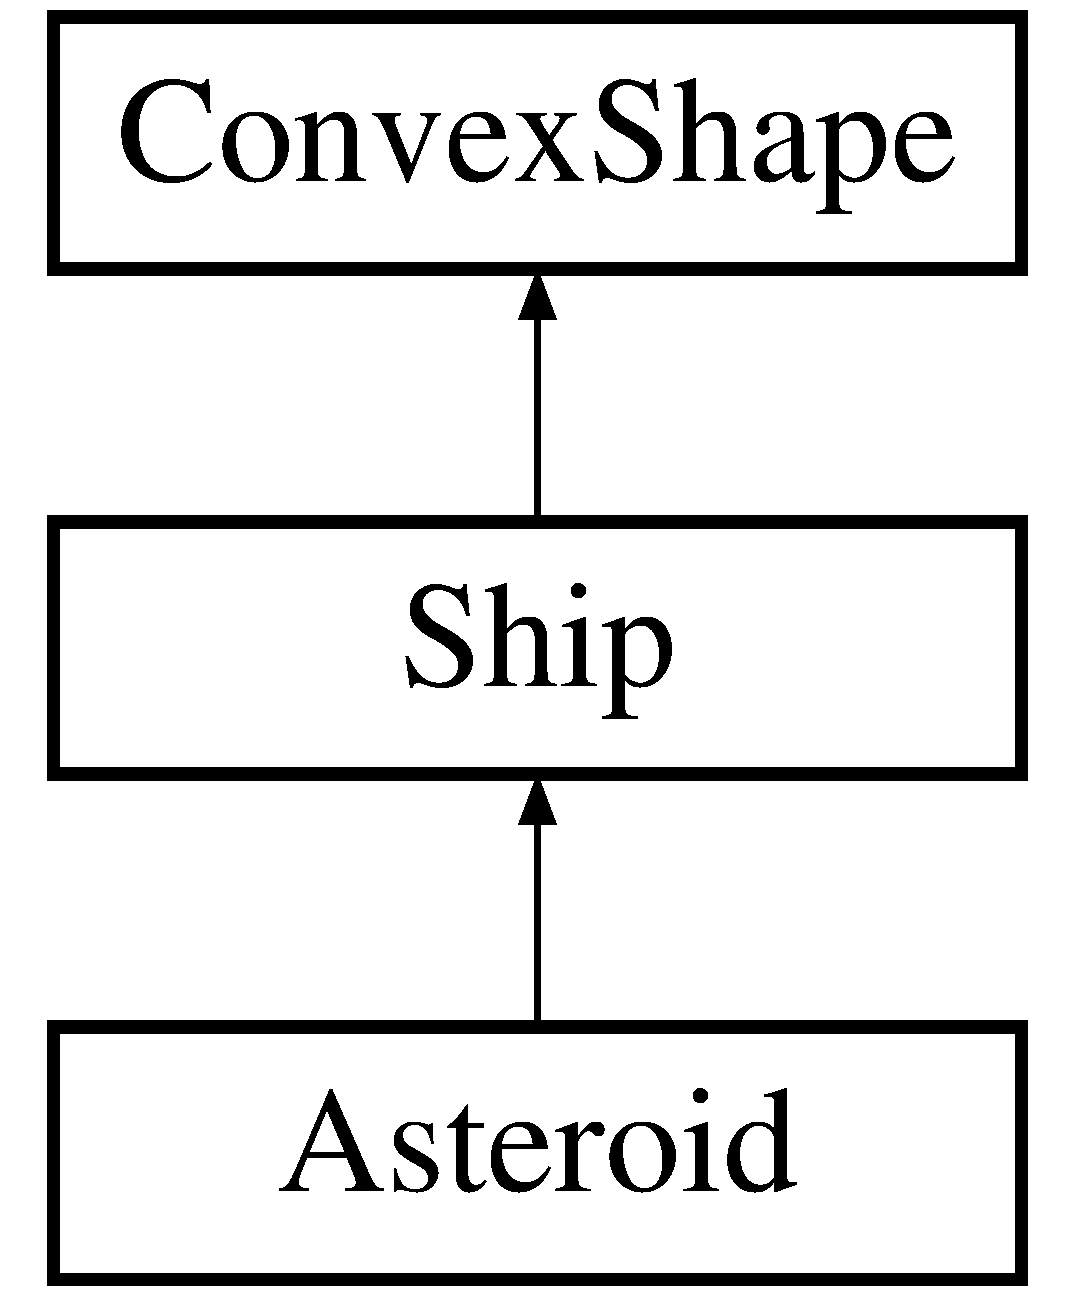
\includegraphics[height=3.000000cm]{class_asteroid}
\end{center}
\end{figure}
\subsection*{Public Member Functions}
\begin{DoxyCompactItemize}
\item 
\hyperlink{class_asteroid_a478e555c280f7f5726e84273d0094dc0}{Asteroid} (sf\+::\+Vector2f const \&position, sf\+::\+Vector2f const \&direction, float spin\+Speed=(rand()\%50-\/25)$\ast$0.\+1f)
\item 
\hypertarget{class_asteroid_af2371381f0daa45c8cba88c9ee04f0a1}{}{\bfseries Asteroid} (sf\+::\+Vector2f const \&position, float spin\+Speed=(rand()\%50-\/25)$\ast$0.\+1f)\label{class_asteroid_af2371381f0daa45c8cba88c9ee04f0a1}

\item 
\hypertarget{class_asteroid_aabe3a75b05df4749a69469a1204b8382}{}void \hyperlink{class_asteroid_aabe3a75b05df4749a69469a1204b8382}{update} () override\label{class_asteroid_aabe3a75b05df4749a69469a1204b8382}

\begin{DoxyCompactList}\small\item\em Moves us forward and keps us spinning. \end{DoxyCompactList}\item 
void \hyperlink{class_asteroid_a1d13470ee5d53dad7dfcbc7ccc56851a}{on\+Collide} (\hyperlink{class_ship}{Ship} $\ast$other) override
\end{DoxyCompactItemize}
\subsection*{Additional Inherited Members}


\subsection{Constructor \& Destructor Documentation}
\hypertarget{class_asteroid_a478e555c280f7f5726e84273d0094dc0}{}\index{Asteroid@{Asteroid}!Asteroid@{Asteroid}}
\index{Asteroid@{Asteroid}!Asteroid@{Asteroid}}
\subsubsection[{Asteroid(sf\+::\+Vector2f const \&position, sf\+::\+Vector2f const \&direction, float spin\+Speed=(rand()\%50-\/25)$\ast$0.\+1f)}]{\setlength{\rightskip}{0pt plus 5cm}Asteroid\+::\+Asteroid (
\begin{DoxyParamCaption}
\item[{sf\+::\+Vector2f const \&}]{position, }
\item[{sf\+::\+Vector2f const \&}]{direction, }
\item[{float}]{spin\+Speed = {\ttfamily (rand()~\%~50~-\/~25)~$\ast$~0.1f}}
\end{DoxyParamCaption}
)}\label{class_asteroid_a478e555c280f7f5726e84273d0094dc0}

\begin{DoxyParams}{Parameters}
{\em position} & Initial position of the \hyperlink{class_asteroid}{Asteroid}. \\
\hline
{\em direction} & The heading that the \hyperlink{class_asteroid}{Asteroid} will travel on  How fast (in degrees per tick) that the asteroid will rotate \\
\hline
\end{DoxyParams}


\subsection{Member Function Documentation}
\hypertarget{class_asteroid_a1d13470ee5d53dad7dfcbc7ccc56851a}{}\index{Asteroid@{Asteroid}!on\+Collide@{on\+Collide}}
\index{on\+Collide@{on\+Collide}!Asteroid@{Asteroid}}
\subsubsection[{on\+Collide(\+Ship $\ast$other) override}]{\setlength{\rightskip}{0pt plus 5cm}void Asteroid\+::on\+Collide (
\begin{DoxyParamCaption}
\item[{{\bf Ship} $\ast$}]{other}
\end{DoxyParamCaption}
)\hspace{0.3cm}{\ttfamily [override]}, {\ttfamily [virtual]}}\label{class_asteroid_a1d13470ee5d53dad7dfcbc7ccc56851a}
Empty method. Does nothing on collision. \begin{DoxyRemark}{Remarks}
Perhaps asteroids should bounce off each other? 
\end{DoxyRemark}


Implements \hyperlink{class_ship}{Ship}.



The documentation for this class was generated from the following files\+:\begin{DoxyCompactItemize}
\item 
Arnieboids/include/Asteroid.\+hpp\item 
Arnieboids/src/Asteroid.\+cpp\end{DoxyCompactItemize}

\hypertarget{class_bullet}{}\section{Bullet Class Reference}
\label{class_bullet}\index{Bullet@{Bullet}}
Inheritance diagram for Bullet\+:\begin{figure}[H]
\begin{center}
\leavevmode
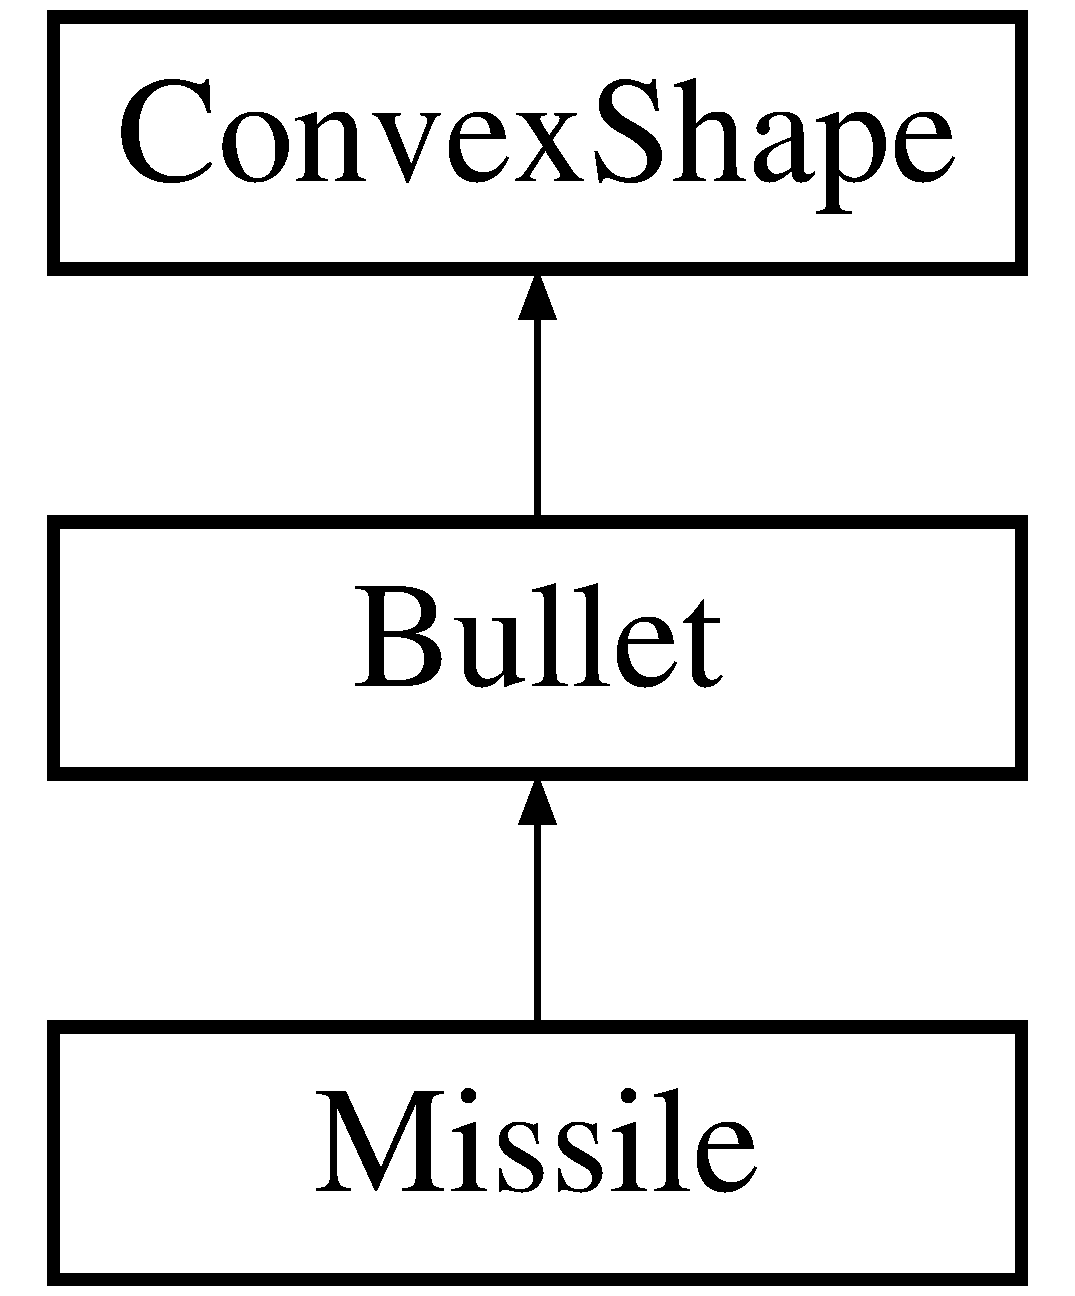
\includegraphics[height=3.000000cm]{class_bullet}
\end{center}
\end{figure}
\subsection*{Public Member Functions}
\begin{DoxyCompactItemize}
\item 
\hypertarget{class_bullet_af049e550cd3848277badd21f86194c49}{}{\bfseries Bullet} (sf\+::\+Vector2f const \&position, sf\+::\+Vector2f const \&direction, const float speed=5.f)\label{class_bullet_af049e550cd3848277badd21f86194c49}

\item 
\hypertarget{class_bullet_a32f4a0611fe2dd245fee955d14ca1f68}{}virtual void \hyperlink{class_bullet_a32f4a0611fe2dd245fee955d14ca1f68}{update} ()\label{class_bullet_a32f4a0611fe2dd245fee955d14ca1f68}

\begin{DoxyCompactList}\small\item\em Moves the bullet forward and checks if it has exceeded time to live. \end{DoxyCompactList}\item 
\hypertarget{class_bullet_ac34da8003c6bc44bddfabce81411bed8}{}bool \hyperlink{class_bullet_ac34da8003c6bc44bddfabce81411bed8}{is\+Active} () const \label{class_bullet_ac34da8003c6bc44bddfabce81411bed8}

\begin{DoxyCompactList}\small\item\em Is the bullet active? \end{DoxyCompactList}\item 
\hypertarget{class_bullet_a3b790871b9487ef3cf5bf956354c8639}{}void {\bfseries set\+Active} (bool active)\label{class_bullet_a3b790871b9487ef3cf5bf956354c8639}

\end{DoxyCompactItemize}
\subsection*{Protected Member Functions}
\begin{DoxyCompactItemize}
\item 
\hypertarget{class_bullet_a27f956e0fe2c7e1da53bff8aecfb87b1}{}float \hyperlink{class_bullet_a27f956e0fe2c7e1da53bff8aecfb87b1}{tick\+To\+Sec} (unsigned int ticks) const \label{class_bullet_a27f956e0fe2c7e1da53bff8aecfb87b1}

\begin{DoxyCompactList}\small\item\em Ticks to seconds. \end{DoxyCompactList}\end{DoxyCompactItemize}
\subsection*{Protected Attributes}
\begin{DoxyCompactItemize}
\item 
\hypertarget{class_bullet_a6fb156b4f69194ca4e6b2c1b23887902}{}float \hyperlink{class_bullet_a6fb156b4f69194ca4e6b2c1b23887902}{speed\+\_\+}\label{class_bullet_a6fb156b4f69194ca4e6b2c1b23887902}

\begin{DoxyCompactList}\small\item\em How far the bullet travels each update. \end{DoxyCompactList}\item 
\hypertarget{class_bullet_a04d2c6f850e61e353b5c84b55f42a6f8}{}unsigned int \hyperlink{class_bullet_a04d2c6f850e61e353b5c84b55f42a6f8}{ticks\+\_\+}\label{class_bullet_a04d2c6f850e61e353b5c84b55f42a6f8}

\begin{DoxyCompactList}\small\item\em Ticks since bullet has spawned. \end{DoxyCompactList}\item 
\hypertarget{class_bullet_a7bc86024912fd5c74aee5c1de7bb3130}{}sf\+::\+Vector2f \hyperlink{class_bullet_a7bc86024912fd5c74aee5c1de7bb3130}{forward\+\_\+}\label{class_bullet_a7bc86024912fd5c74aee5c1de7bb3130}

\begin{DoxyCompactList}\small\item\em The direction or heading of the bullet. \end{DoxyCompactList}\item 
\hypertarget{class_bullet_ae23efe218426ce94127db9d8baac29dd}{}int {\bfseries life\+Time\+\_\+}\label{class_bullet_ae23efe218426ce94127db9d8baac29dd}

\item 
\hypertarget{class_bullet_a46cc668478d5c798e4cbe85a56f14939}{}bool {\bfseries active\+\_\+}\label{class_bullet_a46cc668478d5c798e4cbe85a56f14939}

\end{DoxyCompactItemize}


The documentation for this class was generated from the following files\+:\begin{DoxyCompactItemize}
\item 
Arnieboids/include/Bullet.\+hpp\item 
Arnieboids/src/Bullet.\+cpp\end{DoxyCompactItemize}

\hypertarget{class_camera}{}\section{Camera Class Reference}
\label{class_camera}\index{Camera@{Camera}}


{\ttfamily \#include $<$Camera.\+hpp$>$}

Inheritance diagram for Camera\+:\begin{figure}[H]
\begin{center}
\leavevmode
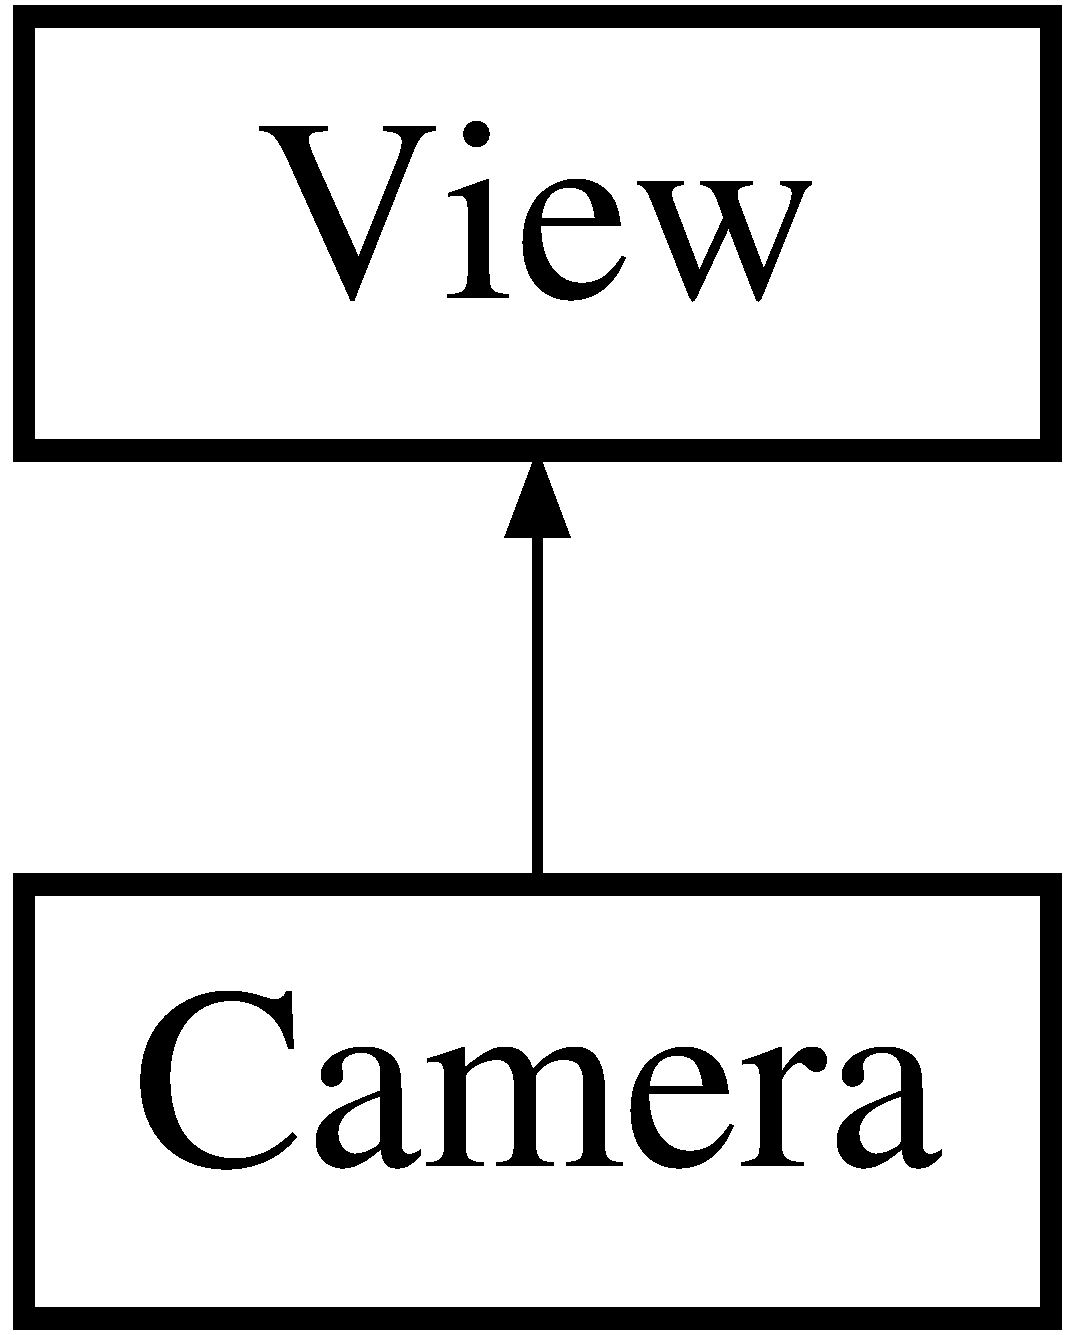
\includegraphics[height=2.000000cm]{class_camera}
\end{center}
\end{figure}
\subsection*{Public Member Functions}
\begin{DoxyCompactItemize}
\item 
\hypertarget{class_camera_a221f2071bdc6218f785bb3b151570c62}{}{\bfseries Camera} (sf\+::\+Vector2u screen\+Size)\label{class_camera_a221f2071bdc6218f785bb3b151570c62}

\item 
\hypertarget{class_camera_abcd03175feb626a823d17d92d55a30d8}{}{\bfseries Camera} (sf\+::\+Vector2u screen\+Size, \hyperlink{class_ship}{Ship} $\ast$target)\label{class_camera_abcd03175feb626a823d17d92d55a30d8}

\item 
\hypertarget{class_camera_a2a8fc39bb84d82d969827d504e4f6928}{}void {\bfseries set\+Target} (\hyperlink{class_ship}{Ship} $\ast$target)\label{class_camera_a2a8fc39bb84d82d969827d504e4f6928}

\item 
\hypertarget{class_camera_ad9ab2d09758faec8de60205b4cecacd9}{}\hyperlink{class_ship}{Ship} $\ast$ {\bfseries get\+Target} ()\label{class_camera_ad9ab2d09758faec8de60205b4cecacd9}

\item 
\hypertarget{class_camera_a2c2eb9907441db681f3fbd34694d415e}{}void {\bfseries clear\+Target} ()\label{class_camera_a2c2eb9907441db681f3fbd34694d415e}

\item 
void \hyperlink{class_camera_a42cda7239981a5618660d04bd5893556}{update} ()
\item 
\hypertarget{class_camera_a8414e6d74d3f6259fa5ea1f037e9d8bd}{}void \hyperlink{class_camera_a8414e6d74d3f6259fa5ea1f037e9d8bd}{move} ()\label{class_camera_a8414e6d74d3f6259fa5ea1f037e9d8bd}

\begin{DoxyCompactList}\small\item\em Not implemented! \end{DoxyCompactList}\item 
\hypertarget{class_camera_a62d35e87b3eeac9463f43c17b65ef090}{}void \hyperlink{class_camera_a62d35e87b3eeac9463f43c17b65ef090}{zoom\+In} ()\label{class_camera_a62d35e87b3eeac9463f43c17b65ef090}

\begin{DoxyCompactList}\small\item\em Not implemented! \end{DoxyCompactList}\item 
\hypertarget{class_camera_aafc1d985053e11bd553b8a12540a562d}{}void {\bfseries zoom\+Out} ()\label{class_camera_aafc1d985053e11bd553b8a12540a562d}

\item 
\hypertarget{class_camera_a20f8f7cb0ef6591c33e9aacb5539c55c}{}void {\bfseries zoom\+Set} ()\label{class_camera_a20f8f7cb0ef6591c33e9aacb5539c55c}

\item 
\hypertarget{class_camera_a9d6e88df1d8fc3e3209089529751be60}{}void {\bfseries zoom\+Reset} ()\label{class_camera_a9d6e88df1d8fc3e3209089529751be60}

\item 
\hypertarget{class_camera_a293e96ec309365bbbe590140ce1b7828}{}void \hyperlink{class_camera_a293e96ec309365bbbe590140ce1b7828}{draw\+H\+U\+D} ()\label{class_camera_a293e96ec309365bbbe590140ce1b7828}

\begin{DoxyCompactList}\small\item\em Not implemented! \end{DoxyCompactList}\end{DoxyCompactItemize}


\subsection{Detailed Description}
Follow camera that can target a ship Also draws that ship\textquotesingle{}s hp and radar to screen 

\subsection{Member Function Documentation}
\hypertarget{class_camera_a42cda7239981a5618660d04bd5893556}{}\index{Camera@{Camera}!update@{update}}
\index{update@{update}!Camera@{Camera}}
\subsubsection[{update()}]{\setlength{\rightskip}{0pt plus 5cm}void Camera\+::update (
\begin{DoxyParamCaption}
{}
\end{DoxyParamCaption}
)}\label{class_camera_a42cda7239981a5618660d04bd5893556}
Updates camera\textquotesingle{}s center to where the target is May also have some nice tweening later 

The documentation for this class was generated from the following files\+:\begin{DoxyCompactItemize}
\item 
Arnieboids/include/Camera.\+hpp\item 
Arnieboids/src/Camera.\+cpp\end{DoxyCompactItemize}

\hypertarget{class_collision_system}{}\section{Collision\+System Class Reference}
\label{class_collision_system}\index{Collision\+System@{Collision\+System}}
\subsection*{Public Member Functions}
\begin{DoxyCompactItemize}
\item 
\hypertarget{class_collision_system_ae4462bc260f16652e5af659164109736}{}{\bfseries Collision\+System} (std\+::list$<$ \hyperlink{class_ship}{Ship} $\ast$ $>$ \&ship\+List, std\+::list$<$ \hyperlink{class_bullet}{Bullet} $\ast$ $>$ \&bullet\+List)\label{class_collision_system_ae4462bc260f16652e5af659164109736}

\item 
\hypertarget{class_collision_system_a0ea99c0b3b16a7df82aad2cb43ecd422}{}void {\bfseries Check} () const \label{class_collision_system_a0ea99c0b3b16a7df82aad2cb43ecd422}

\end{DoxyCompactItemize}


The documentation for this class was generated from the following files\+:\begin{DoxyCompactItemize}
\item 
Arnieboids/include/Collision\+System.\+hpp\item 
Arnieboids/src/Collision\+System.\+cpp\end{DoxyCompactItemize}

\hypertarget{class_game}{}\section{Game Class Reference}
\label{class_game}\index{Game@{Game}}


{\ttfamily \#include $<$Game.\+hpp$>$}

\subsection*{Public Member Functions}
\begin{DoxyCompactItemize}
\item 
\hypertarget{class_game_a50d0ebb6c8c0dbb762d2c1c10bc0c91c}{}{\bfseries Game} (unsigned int win\+Width=800\+U, unsigned int win\+Height=600\+U, unsigned int time\+Per\+Tick=16\+U)\label{class_game_a50d0ebb6c8c0dbb762d2c1c10bc0c91c}

\item 
\hypertarget{class_game_a99fb161fbbe87d25a8b73265a0611e58}{}int \hyperlink{class_game_a99fb161fbbe87d25a8b73265a0611e58}{run} ()\label{class_game_a99fb161fbbe87d25a8b73265a0611e58}

\begin{DoxyCompactList}\small\item\em Implements the main game loop. While window\+\_\+ is open\+: Calls handle\+Events(), Implements a fixed timestep and calls update() and draw() inside it. \end{DoxyCompactList}\end{DoxyCompactItemize}


\subsection{Detailed Description}
Updates and draws all ships and bullets. Culls dead bullets and ships.

\begin{DoxyRemark}{Remarks}
Chrono members are used for fixed timestep 
\end{DoxyRemark}


The documentation for this class was generated from the following files\+:\begin{DoxyCompactItemize}
\item 
Arnieboids/include/Game.\+hpp\item 
Arnieboids/src/Game.\+cpp\end{DoxyCompactItemize}

\hypertarget{class_key_input}{}\section{Key\+Input Class Reference}
\label{class_key_input}\index{Key\+Input@{Key\+Input}}


{\ttfamily \#include $<$Key\+Input.\+hpp$>$}

\subsection*{Public Member Functions}
\begin{DoxyCompactItemize}
\item 
\hypertarget{class_key_input_ab32b8ec028e37e27e059c0ba5109d9f0}{}void \hyperlink{class_key_input_ab32b8ec028e37e27e059c0ba5109d9f0}{update} ()\label{class_key_input_ab32b8ec028e37e27e059c0ba5109d9f0}

\begin{DoxyCompactList}\small\item\em Updates all keys. \end{DoxyCompactList}\item 
\hypertarget{class_key_input_a14646d6a26aac7f82877b6f14a860810}{}bool \hyperlink{class_key_input_a14646d6a26aac7f82877b6f14a860810}{is\+Key\+Down} (const Key key) const \label{class_key_input_a14646d6a26aac7f82877b6f14a860810}

\begin{DoxyCompactList}\small\item\em Is a key down. \end{DoxyCompactList}\item 
\hypertarget{class_key_input_a05667656783ac709b9b2aaf22f2eab93}{}bool \hyperlink{class_key_input_a05667656783ac709b9b2aaf22f2eab93}{is\+Key\+Up} (const Key key) const \label{class_key_input_a05667656783ac709b9b2aaf22f2eab93}

\begin{DoxyCompactList}\small\item\em Is a key up. \end{DoxyCompactList}\item 
\hypertarget{class_key_input_aedc341260ca4a091ae068c9511fc2060}{}bool \hyperlink{class_key_input_aedc341260ca4a091ae068c9511fc2060}{is\+Key\+Pressed} (const Key key) const \label{class_key_input_aedc341260ca4a091ae068c9511fc2060}

\begin{DoxyCompactList}\small\item\em Has a key just been pressed. \end{DoxyCompactList}\item 
\hypertarget{class_key_input_abc5ff40ae7764fc2aa9694a5d5b46fb6}{}bool \hyperlink{class_key_input_abc5ff40ae7764fc2aa9694a5d5b46fb6}{is\+Key\+Released} (const Key key) const \label{class_key_input_abc5ff40ae7764fc2aa9694a5d5b46fb6}

\begin{DoxyCompactList}\small\item\em Has a key just been released. \end{DoxyCompactList}\end{DoxyCompactItemize}


\subsection{Detailed Description}
Holds and handles all key inputs Should be updated with game and then queried for keys 

The documentation for this class was generated from the following files\+:\begin{DoxyCompactItemize}
\item 
Arnieboids/include/Key\+Input.\+hpp\item 
Arnieboids/include/Key\+Input.\+cpp\end{DoxyCompactItemize}

\hypertarget{class_missile}{}\section{Missile Class Reference}
\label{class_missile}\index{Missile@{Missile}}
Inheritance diagram for Missile\+:\begin{figure}[H]
\begin{center}
\leavevmode
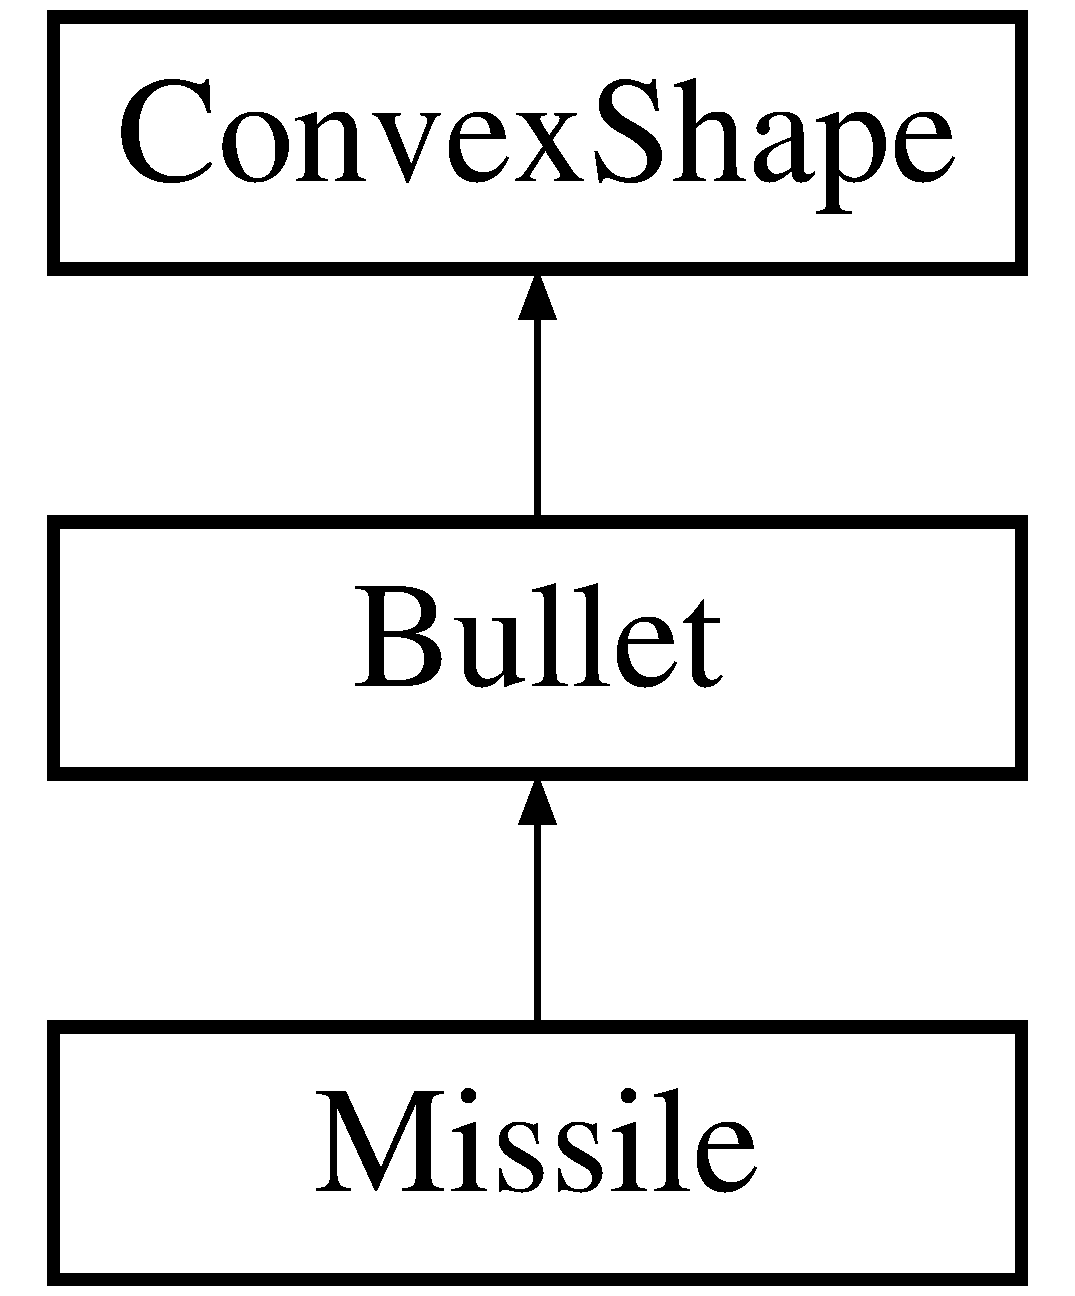
\includegraphics[height=3.000000cm]{class_missile}
\end{center}
\end{figure}
\subsection*{Public Member Functions}
\begin{DoxyCompactItemize}
\item 
\hyperlink{class_missile_aea0c73fed2dbe063cca8dae4e67ce410}{Missile} (const \hyperlink{class_ship}{Ship} $\ast$const target, sf\+::\+Vector2f const \&position, sf\+::\+Vector2f const \&direction, const float max\+Speed=5.f, const float acceleration=0.\+1f, const float turn\+Speed=2.\+f)
\item 
\hypertarget{class_missile_a6bc00954b20db86b293fd4d98012cd09}{}virtual void \hyperlink{class_missile_a6bc00954b20db86b293fd4d98012cd09}{update} () override\label{class_missile_a6bc00954b20db86b293fd4d98012cd09}

\begin{DoxyCompactList}\small\item\em Turns to face target while thrusting forward. \end{DoxyCompactList}\end{DoxyCompactItemize}
\subsection*{Protected Attributes}
\begin{DoxyCompactItemize}
\item 
\hypertarget{class_missile_ad655d9b73602460ac7f4c7be86feb6dd}{}const \hyperlink{class_ship}{Ship} $\ast$const \hyperlink{class_missile_ad655d9b73602460ac7f4c7be86feb6dd}{T\+A\+R\+G\+E\+T\+\_\+}\label{class_missile_ad655d9b73602460ac7f4c7be86feb6dd}

\begin{DoxyCompactList}\small\item\em \hyperlink{class_ship}{Ship} to be tracked. \end{DoxyCompactList}\item 
\hypertarget{class_missile_ab1c0fd40b3e3ab420ec4402e427037b6}{}const float \hyperlink{class_missile_ab1c0fd40b3e3ab420ec4402e427037b6}{M\+A\+X\+\_\+\+S\+P\+E\+E\+D\+\_\+}\label{class_missile_ab1c0fd40b3e3ab420ec4402e427037b6}

\begin{DoxyCompactList}\small\item\em Maximum speed of the missile. Higher value == larger turning circle. \end{DoxyCompactList}\item 
\hypertarget{class_missile_abf37317e40a4a9c947ee868edb7db135}{}const float \hyperlink{class_missile_abf37317e40a4a9c947ee868edb7db135}{A\+C\+C\+E\+L\+E\+R\+A\+T\+I\+O\+N\+\_\+}\label{class_missile_abf37317e40a4a9c947ee868edb7db135}

\begin{DoxyCompactList}\small\item\em How fast (per tick) the missile accelerates. \end{DoxyCompactList}\item 
\hypertarget{class_missile_a78806f677e77faa9b24a23962798ee7f}{}const float \hyperlink{class_missile_a78806f677e77faa9b24a23962798ee7f}{T\+U\+R\+N\+\_\+\+S\+P\+E\+E\+D\+\_\+}\label{class_missile_a78806f677e77faa9b24a23962798ee7f}

\begin{DoxyCompactList}\small\item\em Has quickly the missile can turn. Higher value == tighter turning circle. \end{DoxyCompactList}\item 
\hypertarget{class_missile_a157cb7f39f14587fc49f2d7b75ab68ab}{}bool \hyperlink{class_missile_a157cb7f39f14587fc49f2d7b75ab68ab}{is\+Accelerating\+\_\+}\label{class_missile_a157cb7f39f14587fc49f2d7b75ab68ab}

\begin{DoxyCompactList}\small\item\em True if the missile has yet to reach max speed. \end{DoxyCompactList}\end{DoxyCompactItemize}
\subsection*{Additional Inherited Members}


\subsection{Constructor \& Destructor Documentation}
\hypertarget{class_missile_aea0c73fed2dbe063cca8dae4e67ce410}{}\index{Missile@{Missile}!Missile@{Missile}}
\index{Missile@{Missile}!Missile@{Missile}}
\subsubsection[{Missile(const Ship $\ast$const target, sf\+::\+Vector2f const \&position, sf\+::\+Vector2f const \&direction, const float max\+Speed=5.\+f, const float acceleration=0.\+1f, const float turn\+Speed=2.\+f)}]{\setlength{\rightskip}{0pt plus 5cm}Missile\+::\+Missile (
\begin{DoxyParamCaption}
\item[{const {\bf Ship} $\ast$const}]{target, }
\item[{sf\+::\+Vector2f const \&}]{position, }
\item[{sf\+::\+Vector2f const \&}]{direction, }
\item[{const float}]{max\+Speed = {\ttfamily 5.f}, }
\item[{const float}]{acceleration = {\ttfamily 0.1f}, }
\item[{const float}]{turn\+Speed = {\ttfamily 2.f}}
\end{DoxyParamCaption}
)}\label{class_missile_aea0c73fed2dbe063cca8dae4e67ce410}

\begin{DoxyParams}{Parameters}
{\em target} & The target for the missile \\
\hline
{\em position} & Initial position \\
\hline
{\em direction} & Launch direction \\
\hline
\end{DoxyParams}


The documentation for this class was generated from the following files\+:\begin{DoxyCompactItemize}
\item 
Arnieboids/include/Missile.\+hpp\item 
Arnieboids/src/Missile.\+cpp\end{DoxyCompactItemize}

\hypertarget{class_player}{}\section{Player Class Reference}
\label{class_player}\index{Player@{Player}}
Inheritance diagram for Player\+:\begin{figure}[H]
\begin{center}
\leavevmode
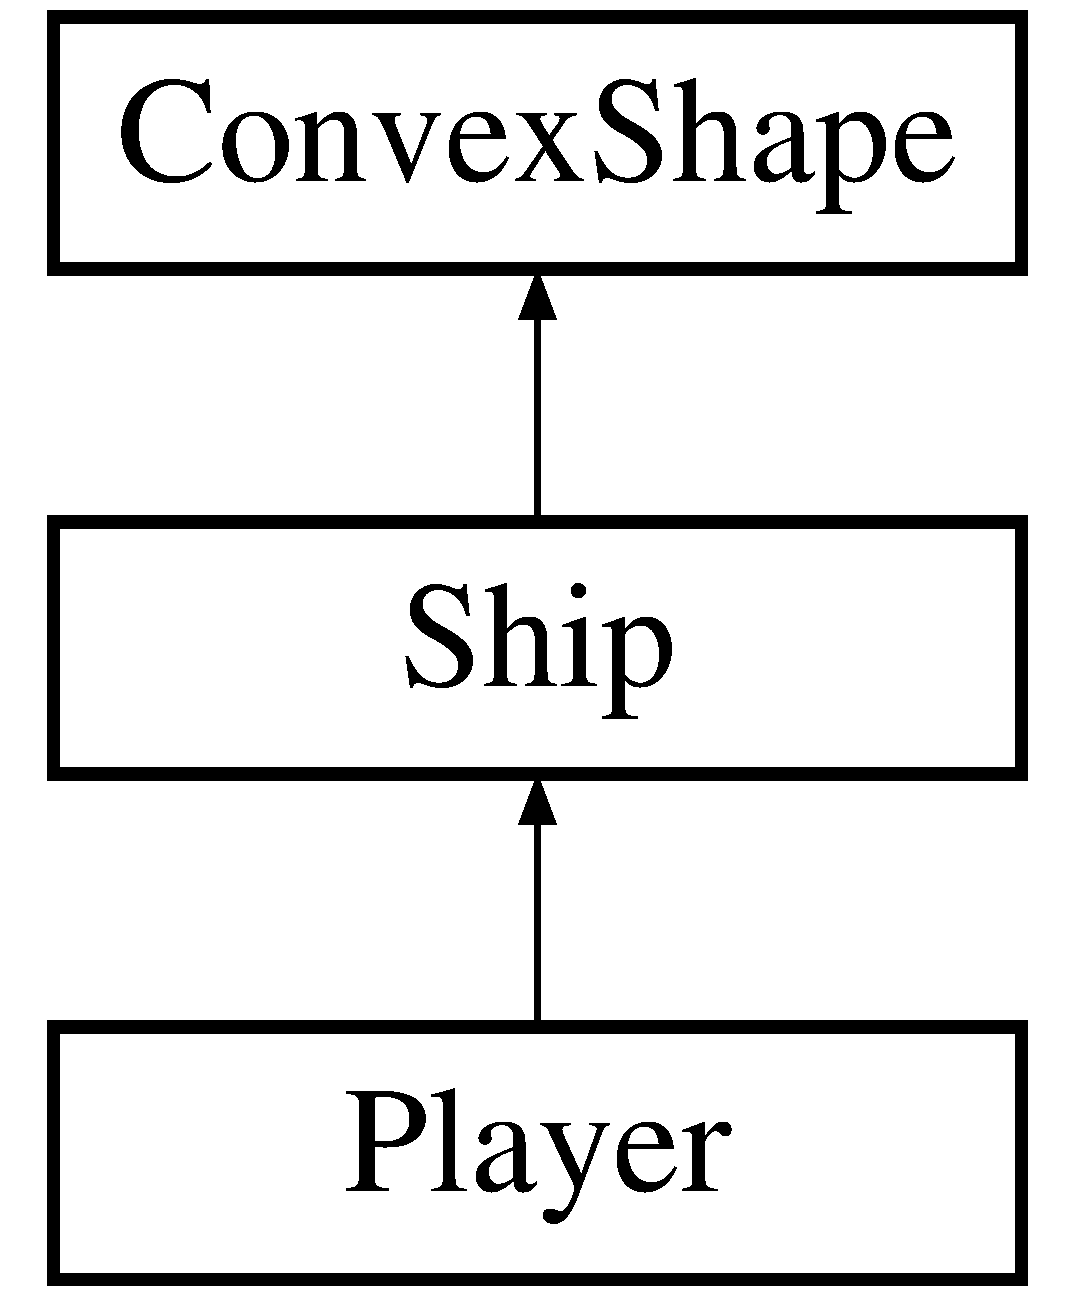
\includegraphics[height=2.000000cm]{class_player}
\end{center}
\end{figure}
\subsection*{Public Member Functions}
\begin{DoxyCompactItemize}
\item 
\hypertarget{class_player_aac1c48b82a1e579cae0f93482f1c6a22}{}{\bfseries Player} (sf\+::\+Vector2f const \&position, unsigned int max\+Health=10\+U)\label{class_player_aac1c48b82a1e579cae0f93482f1c6a22}

\item 
\hypertarget{class_player_a6912bb6e48efb5845d59f0f4582827ef}{}void \hyperlink{class_player_a6912bb6e48efb5845d59f0f4582827ef}{update} () override\label{class_player_a6912bb6e48efb5845d59f0f4582827ef}

\begin{DoxyCompactList}\small\item\em Hides sf\+::\+Shape\+::update() \end{DoxyCompactList}\end{DoxyCompactItemize}


The documentation for this class was generated from the following files\+:\begin{DoxyCompactItemize}
\item 
Arnieboids/include/Player.\+hpp\item 
Arnieboids/src/Player.\+cpp\end{DoxyCompactItemize}

\hypertarget{class_ship}{}\section{Ship Class Reference}
\label{class_ship}\index{Ship@{Ship}}


Base \hyperlink{class_ship}{Ship} class. Abstract class that inherits from sf\+::\+Convex\+Shape. Contains members common to all ships.  




{\ttfamily \#include $<$Ship.\+hpp$>$}

Inheritance diagram for Ship\+:\begin{figure}[H]
\begin{center}
\leavevmode
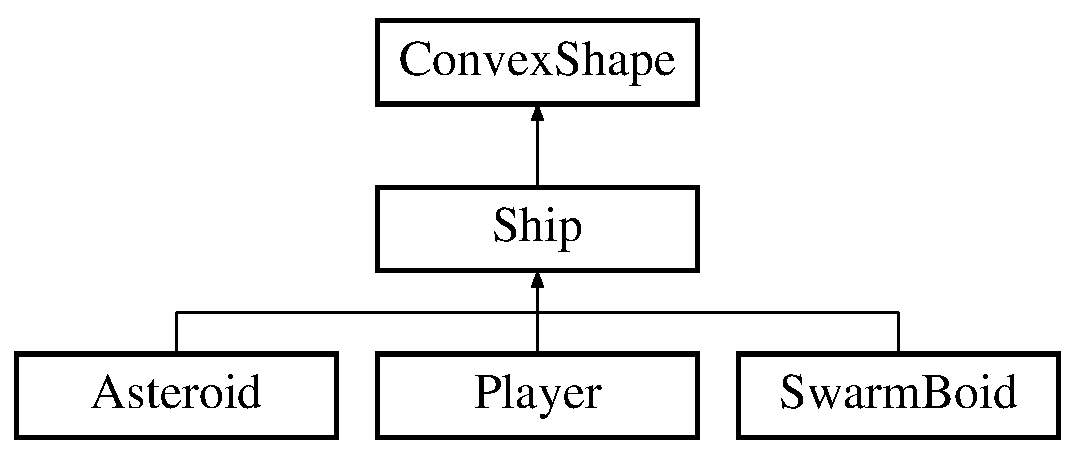
\includegraphics[height=3.000000cm]{class_ship}
\end{center}
\end{figure}
\subsection*{Public Member Functions}
\begin{DoxyCompactItemize}
\item 
\hypertarget{class_ship_a4361703fa6d49a17f080648e1c2dc60b}{}{\bfseries Ship} (float max\+Speed)\label{class_ship_a4361703fa6d49a17f080648e1c2dc60b}

\item 
\hypertarget{class_ship_abfe8b92e7f0346b198e8c40cff44ebeb}{}virtual void \hyperlink{class_ship_abfe8b92e7f0346b198e8c40cff44ebeb}{update} ()=0\label{class_ship_abfe8b92e7f0346b198e8c40cff44ebeb}

\begin{DoxyCompactList}\small\item\em Hides sf\+::\+Shape\+::update() \end{DoxyCompactList}\item 
\hypertarget{class_ship_a966830e20a179ada7d4b7301577b72d7}{}virtual void {\bfseries on\+Collide} (\hyperlink{class_ship}{Ship} $\ast$other)=0\label{class_ship_a966830e20a179ada7d4b7301577b72d7}

\item 
\hypertarget{class_ship_a3a0732b4bb4697b57398cec3b24d76ed}{}void {\bfseries take\+Damage} (unsigned int amount)\label{class_ship_a3a0732b4bb4697b57398cec3b24d76ed}

\item 
\hypertarget{class_ship_a52d219bbadbba6475b919f8e6497ce34}{}bool {\bfseries is\+Dead} () const \label{class_ship_a52d219bbadbba6475b919f8e6497ce34}

\end{DoxyCompactItemize}
\subsection*{Protected Member Functions}
\begin{DoxyCompactItemize}
\item 
\hypertarget{class_ship_a8e7bc2ee7d749ab0d28062091733987c}{}void \hyperlink{class_ship_a8e7bc2ee7d749ab0d28062091733987c}{clamp\+To\+Max\+Speed} ()\label{class_ship_a8e7bc2ee7d749ab0d28062091733987c}

\begin{DoxyCompactList}\small\item\em Clamps the length of the velocity\+\_\+ vector to M\+A\+X\+\_\+\+S\+P\+E\+E\+D\+\_\+. \end{DoxyCompactList}\end{DoxyCompactItemize}
\subsection*{Protected Attributes}
\begin{DoxyCompactItemize}
\item 
\hypertarget{class_ship_a6843554ddc3c0098bcc9d17f7a7fbf3b}{}const float \hyperlink{class_ship_a6843554ddc3c0098bcc9d17f7a7fbf3b}{M\+A\+X\+\_\+\+S\+P\+E\+E\+D\+\_\+}\label{class_ship_a6843554ddc3c0098bcc9d17f7a7fbf3b}

\begin{DoxyCompactList}\small\item\em Maximum length of velocity\+\_\+ vector. \end{DoxyCompactList}\item 
\hypertarget{class_ship_ac1584ef024d6ed1538eb2d1e99661557}{}sf\+::\+Vector2f \hyperlink{class_ship_ac1584ef024d6ed1538eb2d1e99661557}{velocity\+\_\+}\label{class_ship_ac1584ef024d6ed1538eb2d1e99661557}

\begin{DoxyCompactList}\small\item\em Change of position of ship per update. \end{DoxyCompactList}\item 
\hypertarget{class_ship_a6a377507ab7c9c91356869121a84c252}{}unsigned int {\bfseries health\+\_\+}\label{class_ship_a6a377507ab7c9c91356869121a84c252}

\end{DoxyCompactItemize}


\subsection{Detailed Description}
Base \hyperlink{class_ship}{Ship} class. Abstract class that inherits from sf\+::\+Convex\+Shape. Contains members common to all ships. 

The documentation for this class was generated from the following files\+:\begin{DoxyCompactItemize}
\item 
Arnieboids/include/Ship.\+hpp\item 
Arnieboids/src/Ship.\+cpp\end{DoxyCompactItemize}

\hypertarget{class_star}{}\section{Star Class Reference}
\label{class_star}\index{Star@{Star}}
Inheritance diagram for Star\+:\begin{figure}[H]
\begin{center}
\leavevmode
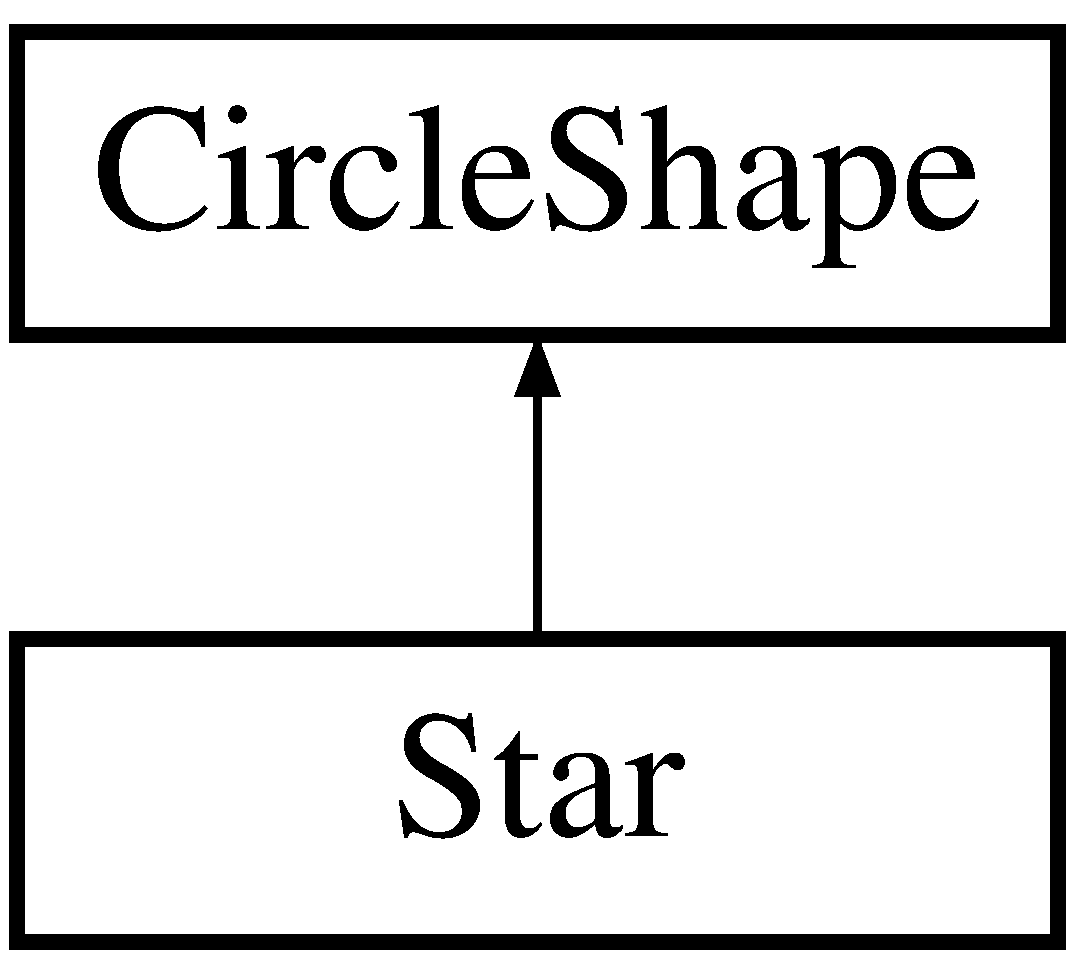
\includegraphics[height=2.000000cm]{class_star}
\end{center}
\end{figure}
\subsection*{Public Member Functions}
\begin{DoxyCompactItemize}
\item 
\hypertarget{class_star_aecbfd462227e97463c78b51926f831bb}{}{\bfseries Star} (sf\+::\+Vector2f position, float radius, sf\+::\+Color col)\label{class_star_aecbfd462227e97463c78b51926f831bb}

\end{DoxyCompactItemize}


The documentation for this class was generated from the following files\+:\begin{DoxyCompactItemize}
\item 
Arnieboids/include/Star.\+hpp\item 
Arnieboids/src/Star.\+cpp\end{DoxyCompactItemize}

\hypertarget{class_swarm_boid}{}\section{Swarm\+Boid Class Reference}
\label{class_swarm_boid}\index{Swarm\+Boid@{Swarm\+Boid}}
Inheritance diagram for Swarm\+Boid\+:\begin{figure}[H]
\begin{center}
\leavevmode
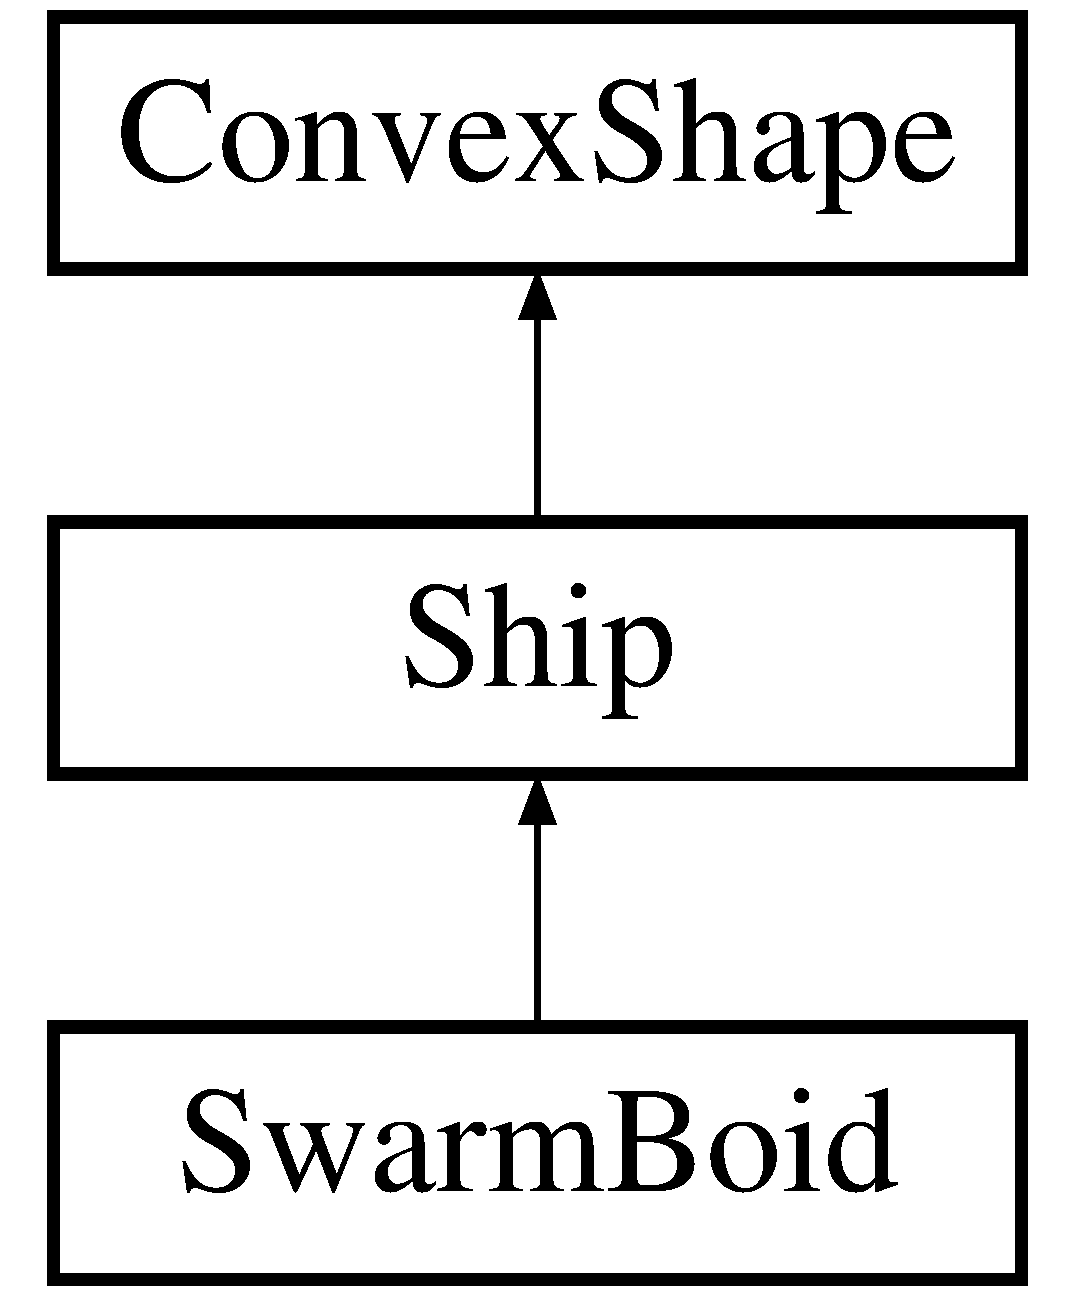
\includegraphics[height=3.000000cm]{class_swarm_boid}
\end{center}
\end{figure}
\subsection*{Public Member Functions}
\begin{DoxyCompactItemize}
\item 
\hypertarget{class_swarm_boid_afbc06919c94d13561f45f5f9c6f59ca4}{}{\bfseries Swarm\+Boid} (sf\+::\+Vector2f position)\label{class_swarm_boid_afbc06919c94d13561f45f5f9c6f59ca4}

\item 
\hypertarget{class_swarm_boid_a25f68c54ca05b761a6aa700801a02cff}{}void \hyperlink{class_swarm_boid_a25f68c54ca05b761a6aa700801a02cff}{update} () override\label{class_swarm_boid_a25f68c54ca05b761a6aa700801a02cff}

\begin{DoxyCompactList}\small\item\em Calls swarm() \end{DoxyCompactList}\item 
\hypertarget{class_swarm_boid_a8268bb58798e2d22d601c88bcaa27bdf}{}void \hyperlink{class_swarm_boid_a8268bb58798e2d22d601c88bcaa27bdf}{on\+Collide} (\hyperlink{class_ship}{Ship} $\ast$other) override\label{class_swarm_boid_a8268bb58798e2d22d601c88bcaa27bdf}

\begin{DoxyCompactList}\small\item\em Takes one damage. \end{DoxyCompactList}\end{DoxyCompactItemize}
\subsection*{Static Public Member Functions}
\begin{DoxyCompactItemize}
\item 
\hypertarget{class_swarm_boid_ad80d43f4292e271fe923e336e4a00fc9}{}static void \hyperlink{class_swarm_boid_ad80d43f4292e271fe923e336e4a00fc9}{set\+Swarm\+Target} (\hyperlink{class_ship}{Ship} $\ast$target)\label{class_swarm_boid_ad80d43f4292e271fe923e336e4a00fc9}

\begin{DoxyCompactList}\small\item\em Sets the target for all swarm boids. They will tend toward this target. \end{DoxyCompactList}\end{DoxyCompactItemize}
\subsection*{Additional Inherited Members}


The documentation for this class was generated from the following files\+:\begin{DoxyCompactItemize}
\item 
Arnieboids/include/Swarm\+Boid.\+hpp\item 
Arnieboids/src/Swarm\+Boid.\+cpp\end{DoxyCompactItemize}

\hypertarget{class_x_controller}{}\section{X\+Controller Class Reference}
\label{class_x_controller}\index{X\+Controller@{X\+Controller}}
\subsection*{Public Member Functions}
\begin{DoxyCompactItemize}
\item 
\hypertarget{class_x_controller_a148116f8235dd69b17f10c09ebc8e493}{}int {\bfseries get\+Port} () const \label{class_x_controller_a148116f8235dd69b17f10c09ebc8e493}

\item 
\hypertarget{class_x_controller_af065f53794859ac0664106a5ff024ef7}{}bool {\bfseries check\+Down} (W\+O\+R\+D button) const \label{class_x_controller_af065f53794859ac0664106a5ff024ef7}

\item 
\hypertarget{class_x_controller_a8f62325ebebceea3c56b164faf9c05cb}{}bool {\bfseries check\+Up} (W\+O\+R\+D button) const \label{class_x_controller_a8f62325ebebceea3c56b164faf9c05cb}

\item 
\hypertarget{class_x_controller_a1cc805edbaecf773f97bfcdbc77a2c4f}{}bool {\bfseries check\+Pressed} (W\+O\+R\+D button) const \label{class_x_controller_a1cc805edbaecf773f97bfcdbc77a2c4f}

\item 
\hypertarget{class_x_controller_a35587b82880720ea2b265d7a7d712190}{}bool {\bfseries check\+Released} (W\+O\+R\+D button) const \label{class_x_controller_a35587b82880720ea2b265d7a7d712190}

\item 
\hypertarget{class_x_controller_aa768bc43116edb8d33ffd4bc83f977fd}{}bool {\bfseries check\+Held} (W\+O\+R\+D button) const \label{class_x_controller_aa768bc43116edb8d33ffd4bc83f977fd}

\item 
\hypertarget{class_x_controller_ad8241a72453c9036b014e6c756bc4468}{}unsigned int {\bfseries check\+Time\+Held} (W\+O\+R\+D button) const \label{class_x_controller_ad8241a72453c9036b014e6c756bc4468}

\item 
\hypertarget{class_x_controller_a62f462d73f5264a0cb468c8d7b3e9da0}{}float {\bfseries check\+Left\+X} () const \label{class_x_controller_a62f462d73f5264a0cb468c8d7b3e9da0}

\item 
\hypertarget{class_x_controller_af78833f9a66c7422c8dd04c32ba35a86}{}float {\bfseries check\+Left\+Y} () const \label{class_x_controller_af78833f9a66c7422c8dd04c32ba35a86}

\item 
\hypertarget{class_x_controller_a99d1ca041e88e230253aaf069246502f}{}float {\bfseries check\+Right\+X} () const \label{class_x_controller_a99d1ca041e88e230253aaf069246502f}

\item 
\hypertarget{class_x_controller_a0eda1afa64aedd18caf7210dfd5fdf77}{}float {\bfseries check\+Right\+Y} () const \label{class_x_controller_a0eda1afa64aedd18caf7210dfd5fdf77}

\item 
\hypertarget{class_x_controller_a97ef1f5e2a9d1cb77f8ebbcdf05cacd9}{}bool {\bfseries check\+Left\+Neutral} () const \label{class_x_controller_a97ef1f5e2a9d1cb77f8ebbcdf05cacd9}

\item 
\hypertarget{class_x_controller_a6650c557d70250cf3b2def17ee068036}{}bool {\bfseries check\+Right\+Neutral} () const \label{class_x_controller_a6650c557d70250cf3b2def17ee068036}

\item 
\hypertarget{class_x_controller_a70320add88de714df1ecc235582d4647}{}int {\bfseries check\+D\+Pad\+X} () const \label{class_x_controller_a70320add88de714df1ecc235582d4647}

\item 
\hypertarget{class_x_controller_ac32d789c025f1eccebfb8edf08541c8f}{}int {\bfseries check\+D\+Pad\+Y} () const \label{class_x_controller_ac32d789c025f1eccebfb8edf08541c8f}

\item 
\hypertarget{class_x_controller_aa9360de1f75371dba977e6dbb9bf17c7}{}float {\bfseries check\+Left\+Trigger} () const \label{class_x_controller_aa9360de1f75371dba977e6dbb9bf17c7}

\item 
\hypertarget{class_x_controller_ab87836fe6d88d4af47f815e686ee4541}{}float {\bfseries check\+Right\+Trigger} () const \label{class_x_controller_ab87836fe6d88d4af47f815e686ee4541}

\item 
\hypertarget{class_x_controller_a59282aca9a7114e6bc64bc082f72fc53}{}bool {\bfseries check\+Left\+Hair\+Trigger} () const \label{class_x_controller_a59282aca9a7114e6bc64bc082f72fc53}

\item 
\hypertarget{class_x_controller_a691089784b0e48d6129235170c1256bb}{}bool {\bfseries check\+Right\+Hair\+Trigger} () const \label{class_x_controller_a691089784b0e48d6129235170c1256bb}

\item 
\hypertarget{class_x_controller_ae52c79dab419e0612bdf60494e9d9576}{}bool {\bfseries set\+Deadzone\+L\+X} (float deadzone)\label{class_x_controller_ae52c79dab419e0612bdf60494e9d9576}

\item 
\hypertarget{class_x_controller_aa993600f76d018dd7710edfd3da3430c}{}bool {\bfseries set\+Deadzone\+L\+Y} (float deadzone)\label{class_x_controller_aa993600f76d018dd7710edfd3da3430c}

\item 
\hypertarget{class_x_controller_a0d3993c8a609e8ea732db7b742ddf22e}{}bool {\bfseries set\+Deadzone\+R\+X} (float deadzone)\label{class_x_controller_a0d3993c8a609e8ea732db7b742ddf22e}

\item 
\hypertarget{class_x_controller_a4106c828fabe8a716f7109723776b5fa}{}bool {\bfseries set\+Deadzone\+R\+Y} (float deadzone)\label{class_x_controller_a4106c828fabe8a716f7109723776b5fa}

\item 
\hypertarget{class_x_controller_aa95c25f438c320aa455a1739191e9bb3}{}bool {\bfseries set\+Threshold\+L\+T} (float threshold)\label{class_x_controller_aa95c25f438c320aa455a1739191e9bb3}

\item 
\hypertarget{class_x_controller_a9fdc050189aa00d922b8101bc9bf5e5d}{}bool {\bfseries set\+Threshold\+R\+T} (float threshold)\label{class_x_controller_a9fdc050189aa00d922b8101bc9bf5e5d}

\item 
\hypertarget{class_x_controller_ab00ba988d215a523a7730f20594fa2c5}{}float {\bfseries get\+Deadzone\+L\+X} () const \label{class_x_controller_ab00ba988d215a523a7730f20594fa2c5}

\item 
\hypertarget{class_x_controller_a705a1d4ad575e6ef15db2391813fd18e}{}float {\bfseries get\+Deadzone\+L\+Y} () const \label{class_x_controller_a705a1d4ad575e6ef15db2391813fd18e}

\item 
\hypertarget{class_x_controller_a08bf17b0a3c086bf5667cf3286cbc585}{}float {\bfseries get\+Deadzone\+R\+X} () const \label{class_x_controller_a08bf17b0a3c086bf5667cf3286cbc585}

\item 
\hypertarget{class_x_controller_abb171d26892efcc9ef5d4109a0e46644}{}float {\bfseries get\+Deadzone\+R\+Y} () const \label{class_x_controller_abb171d26892efcc9ef5d4109a0e46644}

\item 
\hypertarget{class_x_controller_a29521bc4c619301d8448cd9b1fa84bc4}{}float {\bfseries get\+Threshold\+L\+T} () const \label{class_x_controller_a29521bc4c619301d8448cd9b1fa84bc4}

\item 
\hypertarget{class_x_controller_a74406c5161e85934a0a25a11ca44fa96}{}float {\bfseries get\+Threshold\+R\+T} () const \label{class_x_controller_a74406c5161e85934a0a25a11ca44fa96}

\item 
\hypertarget{class_x_controller_addafe067b836a5b5d6cfa6a1d9ff72cb}{}bool {\bfseries update} (int milliseconds)\label{class_x_controller_addafe067b836a5b5d6cfa6a1d9ff72cb}

\end{DoxyCompactItemize}


The documentation for this class was generated from the following files\+:\begin{DoxyCompactItemize}
\item 
Arnieboids/include/X\+Controller.\+hpp\item 
Arnieboids/src/X\+Controller.\+cpp\end{DoxyCompactItemize}

%--- End generated contents ---

% Index
\backmatter
\newpage
\phantomsection
\clearemptydoublepage
\addcontentsline{toc}{chapter}{Index}
\printindex

\end{document}
